\documentclass{article}
\usepackage{amsmath}
\usepackage{setspace}
\usepackage{hyperref}
\usepackage{mathrsfs}
\usepackage{graphicx}
\usepackage[utf8]{inputenc}
\usepackage{tcolorbox}
\usepackage{caption}
 \usepackage{multirow}
 \usepackage{float}
 \restylefloat{table}
 \usepackage{imakeidx}

% Default fixed font does not support bold face
\DeclareFixedFont{\ttb}{T1}{txtt}{bx}{n}{12} % for bold
\DeclareFixedFont{\ttm}{T1}{txtt}{m}{n}{12}  % for normal

% Custom colors
\usepackage{color}
\definecolor{deepblue}{rgb}{0,0,0.5}
\definecolor{deepred}{rgb}{0.6,0,0}
\definecolor{deepgreen}{rgb}{0,0.5,0}

\usepackage{listings}

\graphicspath{ {figures/} }

\tcbuselibrary{minted,breakable,xparse,skins}
\newenvironment{code}{\captionsetup{type=listing}}{}
\definecolor{bg}{gray}{1}
\DeclareTCBListing{mintedbox}{O{}m!O{}}{%
	breakable=true,
	listing engine=minted,
	listing only,
	minted language=#2,
	minted style=default,
	minted options={%
		linenos,
		gobble=0,
		breaklines=true,
		breakafter=,,
		fontsize=\small,
		numbersep=8pt,
		#1},
	boxsep=0pt,
	left skip=0pt,
	right skip=0pt,
	left=25pt,
	right=0pt,
	top=3pt,
	bottom=3pt,
	arc=5pt,
	leftrule=0pt,
	rightrule=0pt,
	bottomrule=2pt,
	toprule=2pt,
	colback=bg,
	colframe=gray!70,
	enhanced,
	overlay={%
		\begin{tcbclipinterior}
			\fill[gray!20!white] (frame.south west) rectangle ([xshift=20pt]frame.north west);
	\end{tcbclipinterior}},
	#3}

\newtcblisting{tcbpythoncode}[1][python]{%
	colback         = gray!5        ,
	colframe        = gray!50!black ,
	listing only                      ,
	title           = #1              ,
	halign title    = right           ,
	fonttitle       = \bfseries       ,
	listing engine  = minted          ,
	minted language = python
}

% Python style for highlighting
\newcommand\pythonstyle{\lstset{
		language=Python.
		basicstyle=\tt\footnotesize,
		otherkeywords={self},             % Add keywords here
		keywordstyle=\bf\color{deepblue},
		emph={MyClass,__init__},          % Custom highlighting
		emphstyle=\bf\color{deepred},    % Custom highlighting style
		stringstyle=\color{deepgreen},
		frame=tb,                         % Any extra options here
		showstringspaces=false,            % 
		breaklines=true
}}


% Python environment
\lstnewenvironment{python, title}[1][]
{
	\pythonstyle
	\lstset{title}
	\lstset{#1}	
}
{}

% Python for external files
\newcommand\pythonexternal[2][]{{
		\pythonstyle
		\lstinputlisting[#1]{#2}}}

% Python for inline
\newcommand\pythoninline[1]{{\pythonstyle\lstinline!#1!}}
\graphicspath{{./figures/}}

%\usepackage[letter,margin=1.5in]{geometry}
%\addtolength{\rightmargin}{-0.5in}
%\addtolength{\textwidth}{0.5in}
%\addtolength{\oddsidemargin}{-.875in}
%\addtolength{\evensidemargin}{-.875in}
%\addtolength{\textheight}{1.75in}

\makeatletter
\renewcommand\section{\clearpage\newpage\@startsection {section}{1}{\z@}%
	{-3.5ex \@plus -1ex \@minus -.2ex}%
	{2.3ex \@plus.2ex}%
	{\normalfont\Large\bfseries}}
\makeatother


% Index code
\makeindex

\newcommand{\boldindex}[1]{%
	\textbf{#1}\index{#1}%
}

\renewcommand{\thefigure}{\arabic{section}.\arabic{figure}}


\begin{document}

%==========================================================================
%==========================================================================
% Title pages.

\newcommand{\mytitle}{[title]}
\newcommand{\myauthor}{Reece Humphreys}
\newcommand{\myadvisor}{Dr. Yaouen Fily}

\newcommand{\myskip}{\vspace{0.5in}}
\newcommand{\layouttitle}[1]{{\bf\large\MakeUppercase{#1}}}
\setlength{\parindent}{0em}
\doublespace
\pagenumbering{roman}
\thispagestyle{empty}

\begin{center}

	\vspace{4in} 
	\layouttitle{\mytitle} \\ by \\ \myauthor
	
	\vspace{1in}
	A Thesis Submitted to the Faculty of \\
	The Wilkes Honors College \\
	in Partial Fulfillment of the Requirements for the Degree of \\
	Bachelor of Science in Liberal Arts and Sciences \\
	with a Concentration in Physics \\ 
	\vspace{1in} 
	Wilkes Honors College of \\
	Florida Atlantic University \\
	Jupiter, Florida \\
	May \number\year

\end{center}

\newpage

%==========================================================================

\vspace{4in}
\begin{center}
	\layouttitle{\mytitle} \\
	by \\
	\myauthor
\end{center}

\singlespace
\vspace{1in}
This thesis was prepared under the direction of the candidate's thesis advisor, \myadvisor, and has been approved by the members of their supervisory committee. It was submitted to the faculty of the Harriet L. Wilkes Honors College and was accepted in partial fulfillment of the requirements for the degree of Bachelor of Science in Liberal Arts and Sciences.

\vspace{1in}
SUPERVISORY COMMITTEE:

\newcommand{\myrule}{\vspace{0.5in}\rule{4in}{0.5pt} \\}

\myrule
\myadvisor

\myrule 
{}[second reader]

\myrule
Interim Dean Timothy Steigenga, Harriet L. Wilkes Honors College 

\myrule
Date

\newpage

%==========================================================================

%\begin{center}
%	\layouttitle{Acknowledgements}
%\end{center}
%\section*{Acknowledgments}
%\addcontentsline{toc}{section}{Acknowledgements}

\myskip
%Some acknowledgments.

\newpage

%==========================================================================

%\begin{center}
%	\layouttitle{Abstract}
%\end{center}
\section*{Abstract}
\addcontentsline{toc}{section}{Abstract}

\myskip
\renewcommand{\arraystretch}{1.5}
\begin{tabular}{@{}l@{\hspace{3ex}}l}
	Author: & \myauthor \\
	Title: & \mytitle \\
	Institution: & Harriet L. Wilkes Honors College, Florida Atlantic University \\
	Thesis Advisor: & \myadvisor \\
	Degree: & Bachelor of Science in Liberal Arts and Sciences \\
	Concentration: & Mathematics \\
	Year: & \the\year
\end{tabular}


\myskip
\doublespace
Orbital debris has quickly become one of the newest sources of pollution as a result of mankind's desire to work in, explore, and utilize space. However, unlike most types of pollution which people experience daily, this is pollution that is impossible for the average person to ever encounter, yet poses just as grand of a threat as the other types. Orbital debris are the remnants of orbital collisions, weapons tests, decommissioned satellites, and spent rocket stages that are passing over our heads faster than bullets and containing similar energy to hand grenades. This paper explores the existing models of orbital debris generation, how clouds of debris evolve with respect to time, and the ramifications that they pose.
\singlespace
\newpage

%==========================================================================

\tableofcontents

%\listoftables
\listoffigures


%==========================================================================

\setlength{\parindent}{1em}
\pagenumbering{arabic}

%==========================================================================
%==========================================================================
% Thesis proper.


\section{Introduction}
\label{introduction}
\doublespace
\subsection{Motivation}
Due to the accelerating launch cadence in the space sector, increased accessibility and resources for small teams to create cube satellites, and satellite mega constellation constructions underway, researchers have become increasingly concerned about the implications of potential orbital collisions. These worries have been compounded by the actions taken by foreign nations with regards to anti-satellite weapons which create substantial amounts of debris. In one such instance, a 2007 Chinese anti-satellite missile test was universally condemned and received statements from government officials such as U.K. prime minister who stated "We are concerned about the impact of debris in space and we expressed that concern”. These fragmentation events can be difficult to track due to the small size of some of the debris fragments that are generated, yet they can pose a great hazard to other satellites and crewed operations being conducted in space. Tens of millions of pieces of orbital debris currently exist within Low Earth Orbit (LEO) with an average size smaller than 1cm. While minuscule in size, these pieces of debris have an average impact velocity of 10 km/s which generates similar energy to that of an exploding hand grenade. It is, therefore, paramount to study the phenomena that arise within orbital debris clouds to gather methods for mitigating debris cloud formations. Without such a study, the future commercialization of space, the potential for humanity to become a multi-planetary species, and the benefits that the advanced satellites provide researchers will remain in jeopardy.
\subsection{Methodology}
To model how debris clouds propagate over time, a method of simulating the debris generated by a collision or explosion is required. Breakup models use observations of orbital collisions to create statistical models that predict the size, mass, speed, and number of debris pieces generated.  Once these characteristics of each debris piece are obtained, equations of motion can be implemented that account for the significant forces acting on each debris fragment, such as drag and solar radiation, to model how the debris position and velocity will evolve over time. This paper implements the NASA Standard Satellite Breakup Model (Source) to simulate the orbital collisions and gather information regarding the behavior of orbital debris. This was accomplished by utilizing the model to create an implementation in python which has been made \href{https://github.com/ReeceHumphreys/OrbitalDebris}{open source on GitHub} for others wishing to build on the foundations of this research.

Following the implementation of the breakup model, the implementation of dominant orbital perturbations is given. These are forces that act on debris to change their orbits over time and include effects such as atmospheric drag and solar radiation. The optimal way to represent these effects is through changes in orbital parameters, which is an alternate way of expressing the current state of an object rather than using euclidean coordinates $(x,y,z, v_x, v_y, v_z)$ . The benefits of using orbital parameters is explored more in-depth later in the paper.

Finally a case study showing the magnitude of orbital collisions is shown along with an analysis on the potential for the Kessler syndrome to occur given the increase in launch cadence and recent expansions into constructing satellite mega constellations.

  
\subsection{Past research and Roadmap}
*** Include what past researchers have explored and where my research fits in*** \newline
An outline of the roadmap for this paper is as follows: \newline 
\textbf{Chapter 1:}  \newline 
\textbf{Chapter 2:}  \newline 
\textbf{Chapter 3:}  \newline 
\textbf{Chapter 4:}   \newline 
\singlespace

\section{Modeling Satellite Breakups}
\label{Modeling Satellite Breakups}
\doublespace


\subsection{The NASA Standard Satellite Breakup Model}

A satellite is any artificial body placed in orbit around the earth or moon or another planet. The definition of the term is intentionally general and as such, can be used to reference space craft (SC), remnants of rockets (RB), and communication devices (SAT) in orbit.  A satellite breakup model is a mathematical model used to describe the outcome of a a satellite breakup due to an explosion or a collision (Liou, 2012) \cite{jer_chyi_liou_orbital_nodate}.  The outcome of any satellite breakup model should be a set of characteristics that should describe the size, area-to-mass (AM) ratio, and the ejection velocity of each fragment produced in the satellite breakup (Johnson and Krisko, 2001) \cite{johnson_nasas_2001}. The NASA Standard Satellite Breakup Model is an industry standard breakup model developed by NASA and is used by most major space agencies such as the European Space Agency (ESA) and the Japanese Aerospace Exploration Agency (JAXA). The implementation of it was provided by Johnson et. al in 2001 \cite{johnson_nasas_2001} but was later clarified by Kristo in 2011 \cite{krisko_proper_2011}. 

The way that the model works is by using experimental observations performed both on Earth and in orbit to characterize the breakup using statistical distributions. The reason being is breakup events are stochastic, i.e are nondeterministic.  For example, explosions are stochastic, they do not occur the same way every time.  By using a statistical distribution and sampling from it we can more accurately represent the fragments that would be generated during a collision or explosion. For this paper, I will be focusing on how the collision fragments are generated, but it should be noted that the explosion case just involves slightly different parameters in many cases.

\newpage

\subsection{Implementing the NASA Breakup Model}

\subsubsection{Characteristic Length and Number of fragments}

In prior versions of the NASA breakup model, the mass of each piece of debris was used as the independent variable for the various distributions characterizing the collision or explosion (Krisko 2001). The model has since evolved to using the size or characteristic length, $L_c$, which is more directly correlated with experimental data for both on-orbit and terrestrial breakup events. The characteristic length makes the assumption that the debris particles are spherical in nature and have the density of aluminum for objects smaller than 1 cm with a diminishing density for larger debris. 

Due to the stochastic nature of collisions and explosions, debris with the same characteristic length may not have the same characteristics (i.e mass, velocity , area). As such, these characteristics are based on distributions that are created using the characteristic length, but the actual value for each debris is randomly sampled from the distribution.

To determine the characteristic lengths that will be used in the simulation, it is crucial to first recognize that collisions and explosions will produce different expressions. Explosions will produce larger debris fragments with smaller velocities while collisions tend to generate a large number of small fragments with high velocities (Barrows, 1996). 

Utilizing the implementation described by Letizia for CiELO, To determine the characteristic length of each piece of debris, first 100 bins are created that are equally spaced on a logarithmic scale between 1mm and 10 cm. Then the number of debris that will be in each bin is computed utilizing the experimental observations of collisions and explosions. Finally to determine the characteristic length of each piece of debris, a randomly sampled value is drawn from the bin that the debris is contained in.
 
\newpage

 \begin{code}
 	\captionof{listing}{Characteristic Lenght Implementation}
 	\begin{tcbpythoncode}
 		def characteristic_lengths(m_target, m_projectile, v_impact, is_catastrophic, debris_type, explosion):
 		bins = np.geomspace(0.001, 0.1, 100)
 		N_fragments = [number_fragments(b, m_target, m_projectile, v_impact, is_catastrophic, debris_type, explosion) for b in bins ]
 		N_fragments = (np.array(N_fragments)).astype(int)
 		
 		L_c = np.concatenate([uniform(bins[i], bins[i+1], size=N_fragments[i]) for i in range(len(bins) - 1)])
 		
 		return L_c
 	\end{tcbpythoncode}
 \end{code}
 
 
 
As mentioned above, since collisions and explosions are fundamentally different, the function that generates the number of debris in a given bin must account for this difference. This is accomplished by specifying whether the given even is a collision or explosion first. In the case that the event is an explosion. The number of explosive fragments of size $L_c$ is governed by the following equation:
$$N(L_c) =S * 6 * L_c^{-1.6}$$
With S = 1, the relationship has been observed to be valid for rocket upper stages with masses in the range of 600-1000 kg (Johnson et al 2001). However, for explosions due to other malfunctions such as battery explosions, anti-satellite tests etc. S having a range between 0.1 to 1 was found to be a good approximate solution where the value of S depends on the explosive body type (Krisko 2001). 

In the case of a collision, a distinction must be made, if the collision was catastrophic or non catastrophic. A collision is categorized as catastrophic if it causes the complete fragmentation of both the impactor and the target (Letizia). This occurs when the energy per target mass exceeds $40 J * g^{-1}$(Krisko 2007). The number of produced fragments for a collision is governed by the following :

$$N(L_c [m]) = 0.1 * (M_e)^{0.75} * L_c^{-1.71}$$

\noindent Where $M_e$ is defined as follows: \\
\indent Catastrophic collision: $M_e[kg] = M_t [kg] + M_p[kg]$ \\
\indent Non Catastrophic collision: $M_e[kg] = M_p[kg] **(v_c [km/s] / 1 [km/s])^2$

\noindent $M_t$ is the target mass, $M_p$ is the projectile mass, $v_c$ is the relative impact velocity between the target and the projectile.


 \begin{code}
	\captionof{listing}{Characteristic Lenght Implementation} 
	\begin{tcbpythoncode}
		def number_fragments(l_characteristic, m_target, m_projectile, v_impact, is_catastrophic, debris_type, explosion):
		if explosion == True: 
		return 6*(l_characteristic)**(-1.6) # Can be multiplied by scaling factor S
		else:
		m_ref = 0 	# Defining reference Mass
		if is_catastrophic: m_ref = m_target + m_projectile
		else: m_ref = m_projectile * (v_impact)**2
		return 0.1 * (m_ref)**0.75 * l_characteristic**-1.71
	\end{tcbpythoncode}
\end{code}

\newpage
\subsubsection{Area to Mass Distribution }

The area-to-mass ratio, A/M, for fragments is a distribution that was based on analysis of thousands of fragmentation debris and provides us with a method to gain information that will be crucial when computing the perturbations on each fragment. The discrete distributions were found by using a $\chi^2$ fit to orbital decay characteristics for 1,780 upper stage explosion fragments, and similar data was developed for spacecraft fragments (Johnson et. al). There are three main producers of orbital debris, rocket bodies, R/B, spacecraft, S/C, and small satellites, soc. For simplicity only the soc distribution function is provided in this paper as the scenario that this paper aims to simulate is for a satellite explosion. However, the implementation for rocket bodies and spacecraft is included in the source code.

For small objects, with $L_c < 8$cm, the A/M distribution is expressed as:  $$D_{A/M}(\lambda_c, \chi) = \mathcal{N}(\mu_{A/M}, \sigma_{A/M}(\lambda_c), \chi) $$

\noindent $D_{A/M}$ is the distribution function of $\chi$ as a function of $\lambda_c$, where
\begin{align*}
	 \lambda_c &= \log_{10}(L_c),\\
	 \chi &= \log_{10}(A/M),\\
 \end{align*}

\noindent $\mathcal{N}$ is the normal distribution function with mean $\mu_{A/M}$ and standard deviation $\sigma_{A/M}$, where

\begin{align}
	 \mu_{A/M} &= \begin{cases} 
		-0.3, & \lambda_c\leq -1.75 \\
		-0.3 - 1.4(\lambda_c + 1.75), & -1.75 < \lambda_c <-1.25 \\
		-1.0, & \lambda_c \geq -1.25 
	\end{cases}\\
	\sigma_{A/M} &= \begin{cases} 
		0.2, & \lambda_c \leq -3.5 \\
		0.2 + 0.1333(\lambda_c + 3.5) & \lambda_c > -3.5 \\
	\end{cases}
\end{align}

Every fragment of debris has a corresponding A/M distribution since both $\mu_{A/M}$ and $\sigma_{A/M}$ are functions of $\lambda_c$. To determine the corresponding A/M ratio for each debris, a random value is drawn from the distribution. This accounts for explosions and collisions not producing the stochastic nature of fragmentation.

Below, the implementation of the A/M distribution is provided in python for the SOC case. Note that the \mintinline{Python}{mean_factory}
and the  \mintinline{Python}{std_dev_factory} function calls are to generate the mean and standard deviation for any debris type, not just SOC. However, the below implementation only demonstrates its application for SOC. The full implementation is included in the open source code base. 

\newpage
 
\begin{code}
	\captionof{listing}{Characteristic Length Implementation} 
	\begin{tcbpythoncode}
		def distribution_AM(lambda_c, debris_type):
		N = len(lambda_c)
		lambda_c = np.array(lambda_c)
		# Generates mu_AM and sigma_AM depending on type of object (RB, SC, SOC)
		mean_factory = make_mean_AM(debris_type)
		std_dev_factory = make_standard_dev_AM(debris_type)
		mean_preSwitch = np.array(mean_factory(lambda_c)) 
		std_dev_preSwitch = np.array(std_dev_factory(lambda_c))
		switch = np.random.uniform(0,1, N)
		# Pulling a random value from the distribution
		means = mean_preSwitch[0]
		devs = std_dev_preSwitch[0]
		return np.random.normal(means, devs, N)
	\end{tcbpythoncode}
\end{code}

The average cross-sectional area, A, also can be obtained through a one-to-one correspondence with $L_c$ using the following expression:
\begin{align}
	A_x = \begin{cases}
		0.540424 * L_c^2 & \text{where } L_c < 0.00167 m \\
		0.556945 * L_c^{2.0047077} & \text{where } L_c \geq 0.00167 m \\
	\end{cases}
\end{align}

\begin{code}
	\captionof{listing}{Characteristic Length Implementation} 
	\begin{tcbpythoncode}
		def avg_area(L_c):
		if L_c < 0.00167: #(m)
		return 0.540424 * L_c**2
		else:
		return 0.556945 * L_c**2.0047077
	\end{tcbpythoncode}
\end{code}

Since the cross sectional area is known and the area to mass ratio is also known, we can now obtain the mass M simply by $$M = A_x / (A/M)$$

\subsubsection{Change in Velocity Distribution }
\noindent The change in velocity, $\Delta v$, distribution is also a function of the A/M ratio. More specifically it is a lognormal distribution modeled as $$D_{\Delta v}= \mathcal{N}(\mu_{v}(\chi), \sigma_{v}(\chi), \xi)$$

\noindent Where, \begin{align}
	\xi &= \log_{10}(\Delta v)\\
	\chi &= \log_{10}(A/M)\\
	\mu_{v}(\chi) &= 0.2\chi+1.85\\
	 \sigma_{v}(\chi) &= 0.4
\end{align}

\begin{code}
	\captionof{listing}{Characteristic Length Implementation} 
	\begin{tcbpythoncode}
		def distribution_deltaV(kai, v_c, explosion=True):
		N = len(kai)
		mean = mean_deltaV(kai, explosion)
		dev = std_dev_deltaV()
		base = 10
		centered = np.random.normal(0, dev, N)
		I = np.nonzero(base**(mean+centered)>1.3*v_c)[0]
		n = len(I)
		while n != 0:
			centered[I] = np.random.normal(0, dev, n)
			#I = np.nonzero(base**(mean+centered)>1.3*v_c)[0]
			J = np.nonzero(base**(mean[I] + centered[I]) >1.3*v_c)[0]
			I = I[J]
			n = len(I)
		
		return base**centered
	\end{tcbpythoncode}
\end{code}

\newpage
\subsection{Validating the Implementation}
Due to the niche nature of orbital debris analysis, it can generally be challenging to find any full implementation of the breakup model. Additionally, many of various space agencies around the world do not share the details of how they implemented the models. For this reason, the above implementations were largely modeled after the details given in the CiELO (Latizia) which mimicks the information provided in NASA literature.

To validate that the python implementation was performed correctly, a comparison is made to existing data provided by various space agencies for a given scenario. This scenario is a  explosion event with a rocket body that weighs 1000kg and the data was provided by Rossi et. al. in "NASA Breakup Model Implementation Comparison of Results".

As shown in the table below, the data from the various space agencies has some significant differences, especially for the characteristic length in the > 1mm range despite all implementing the same NASA breakup model. This is most likely a result of ambiguities in the original NASA breakup model specification literature as well as differences in how various programming languages perform random sampling. The goal of the python implementation is to be within the original deviations of the data. ... 

\begin{table}[H]
		\noindent\makebox[\textwidth]{
				\begin{tabular}{|lccccccc|}
				\hline
				\multicolumn{1}{|c|}{\multirow{3}{*}{\textbf{Model}}} & \multicolumn{7}{c|}{Number of Fragments}                                                        \\ \cline{2-8} 
				\multicolumn{1}{|c|}{}                                & \multicolumn{4}{c|}{Length}  & \multicolumn{1}{c|}{Mass} & \multicolumn{1}{c|}{Area} & Velocity \\
				\multicolumn{1}{|c|}{} &
				\textgreater 1mm &
				\textgreater 1cm &
				\textgreater 10cm &
				\multicolumn{1}{c|}{\textgreater 1m} &
				\multicolumn{1}{c|}{\textgreater 1g} &
				\multicolumn{1}{c|}{\textgreater 1cm\textasciicircum{}2} &
				\textgreater 100ms\textasciicircum{}-1 \\ \hline
				ASI                                                   & 378,581   & 9,403  & 234 & 7 & 2,472                     & 5,878                     & 112,932  \\
				CNSA                                                  & 37,865    & 960    & 32  & 9 & 254                       & -                         & 11,380   \\
				DLR                                                   & 1,217,054 & 11,724 & 230 & 0 & 25,844                    & 31,124                    & 31,124   \\
				ESA                                                   & 324,886   & 8,159  & 206 & 6 & 2,093                     & 5,024                     & 98,717   \\
				NASA                                                  & 434,928   & 10,731 & 248 & 8 & 2,525                     & 6,416                     & 132,032  \\
				\textit{Python Implementation}                        & -         & -      & -   & - & -                         & -                         & -        \\ \hline
			\end{tabular}
		}
		\caption{(Data Source: NASA Breakup Model Implementation Comparison of results, A. Rossi, 24th IADC Meeting April 2006) }
		\label{tab:debris-comparison}
\end{table}

... \textbf{will elaborate more in this section once the python implementation has been fixed and validated}

\subsection{Application}

... \textbf{will elaborate more in this section once the python implementation has been fixed and validated}

\newpage
\section{State Representation}

Following the successful computation of the fragmentation event, we need to construct the representation of each fragment as a piece of orbital debris. There are two primary methods for representing the state of an orbital body.

The first is using \boldindex{orbital state vectors} to represent the object. Orbital state vectors consist of the Cartesian vector's position, $\vec{r}$, and velocity $\vec{v}$ along with time, t. This representation is a natural result of Newton's laws of motion and the Universal Law of Gravitation.

The second representation is as \boldindex{keplerian elements}, which are a result of Kepler's laws of planetary motion. These consist of the eccentricity, \emph{e}, Semimajor axis, \emph{a}, inclination, \emph{i}, longitude of the ascending node, $\Omega$, the argument of periapsis, $\omega$, and the true anomaly, $\nu$. Keplerian elements are a more abstract representation of the motion of an object, but provide significant benefits are explored in the subsequent subsections. 

The combination of both of these state representations is used as they each pose benefits and drawbacks for conducting a simulation.

\subsection{Orbital State vectors and their advantages}

The Orbital State vectors utilize Newton's laws of motion and Newton's Universal Law of gravitation to describe the motion of an object in space. 
Newton's Universal Law of Gravitation states that $$\vec{F_{grav}} = G\frac{ m_1 m_2 \vec{r}}{\mid\vec{r}\mid^3}$$ \noindent This is the dominant force that will be acting on an orbital object, neglecting drag. As such application of newtons second law yields
\begin{align}
	m_1 * \vec{a_1}  & = G\frac{m_1 m_2 \vec{r}}{\mid\vec{r}\mid^3}\\
	\vec{a_i}  &= G \sum_{i \ne j}  m_j \frac{\vec{r_j} -\vec{r_i}}{\mid\vec{r_j - r_i}\mid^3} \indent\text{(More general)}
\end{align}

As such, the change in an object's velocity can be expressed as the sum of the contributions of gravitational attraction from all other surrounding bodies. Due to the gravitational force depending on mass, the gravitational attraction for a piece of debris to nearby debris is negligible compared to the gravitational attraction from a nearby planetary body. Thus, for computational efficiency, inter-particle interactions will be neglected.

The benefits of using orbital state vectors are that they provide a natural intuition for how the motion of a piece of debris will change over time and they provide the necessary information for doing 3D visualization. However, a large drawback of using state vectors is that all six degrees of freedom, $ (x, y, z, v_x, v_y, v_z)$, will be changing during every timestep. As such when simulating a large number of fragments orbiting a body, the memory usage will grow quite large. Additionally, the periodic nature of orbits is not captured with this parameterization, meaning to know the state of a piece of debris in the far future will require propagating that debris from its initial conditions up to the desired time step. This again is an undesirable consequence and one of the primary motivations for using the Keplerian element parameterization.
 
\newpage
\subsection{Keplerian elements and their advantages}

Viewed from an inertial plane, two orbiting bodies trace distinctive trajectories, where each has a focus at the common center of mass. When switching to a non-inertial frame centered on one of the bodies, only the trajectory of the opposite body is viewable. Keplerian elements are a parameterization that describes these non-inertial trajectories (Wikibook).

The reference body is called the primary, and in our case will be the Earth, while the other body is the secondary. It should be noted that there is no preferred primary or secondary.

To parameterize the motion of the orbital debris using Keplerian Elements the first step is use the position vector, $\vec{r}$, and velocity vector, $\vec{v}$, defined in the above subsection to define the \boldindex{specific angular momentum} vector as follows

\begin{equation}
\vec{h} = \vec{r} \times \vec{v}
\end{equation}

Using the Earths equator as the \boldindex{fundamental plane}, which is the plane that is used as a reference, we can begin constructing the parameters of the \boldindex{orbital plane}, which is the plane created by tracing out the $\vec{r}$ vector, which contains both the $\vec(r)$ vector and $\vec{v}$ vector. The intersection of the orbital plane with the fundamental plane is called the \boldindex{line of nodes}

The \boldindex{ascending node} is the spot where the orbiting body crosses the plane of reference / equatorial plane in a northerly direction. Similarly, the \boldindex{descending node} is where it crosses the plane of reference in a southerly direction. $\vec{n}$ is a vector that points in the direction of the ascending node and is found by taking the cross product of the unit vector $\hat{k}$ with the angular momentum $\vec{h}$

\begin{equation}
\vec{n} = \hat{k} \times \vec{h}
\end{equation}

\begin{figure}[t]
	\centering
	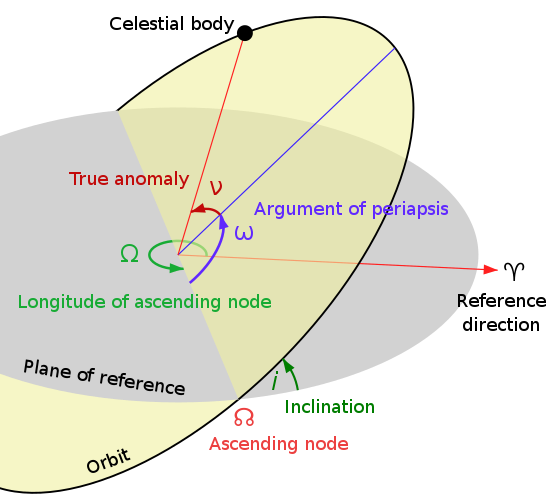
\includegraphics[scale=0.35]{keplerian-elements}
	\caption{A figure}
\end{figure}

Using the parameters typically used for specifying an ellipse, we can also describe an orbit

The \boldindex{Semi-Major Axis}, a,  is one half of the major axis. The major axis is a line that goes through both foci of the ellipse and the center, and ends at the widest point of the perimeter.

\begin{figure}[h]
	\centering
	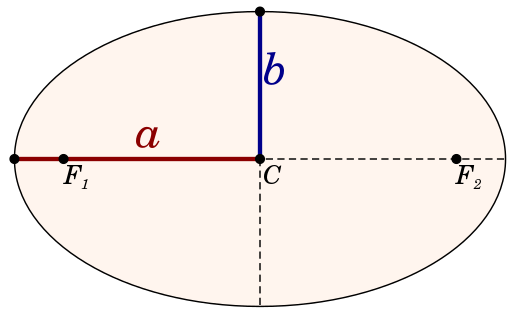
\includegraphics[scale=0.35]{semi-major_and_minor_axes}
	\caption{A figure}
\end{figure}

Using the Vis-Viva equation, the semi-major axis, a, can be defined as:
\begin{equation}
a = \frac{1}{\frac{2}{\mid \vec{r} \mid} - \frac{\mid \vec{v} \mid^2 }{\mu}}
\end{equation}
\noindent where $\mu$ is the standard gravitational parameter of the primary body. For Earth the value of $\mu$ is $\mu = 3.986 *10^{14} \frac{m^3}{s^2}$.

The \boldindex{orbital eccentricity} is a dimensionless parameter that indicates to what degree an orbit around another body deviates from a perfect circle. It has the value of 0 for a circular orbit, a value between 0 and 1 for elliptic orbits, 1 fir parabolic escape orbits, and greater than 1 for hyperbolic orbits. For the purpose of orbital debris in LEO, the eccentricities will be in the elliptic orbit range.

The equation for eccentricity can be expressed from the the Orbital State vectors as follows:
\begin{equation}
\vec{e} = (\frac{\mid \vec{v} \mid^2}{\mu} - \frac{1}{\mid \vec{r} \mid})\vec{r} - \frac{(\vec{r} \cdot \vec{v})}{\mu}\vec{v}
\end{equation}

\begin{figure}[h]
	\centering
	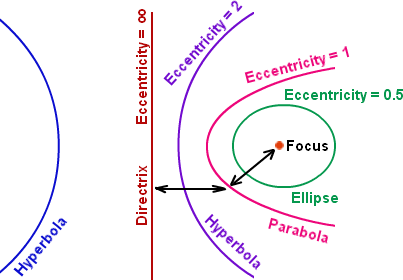
\includegraphics[scale=0.45]{eccentricity}
	\caption{A figure}
\end{figure}

The \boldindex{inclination}, \textit{i}, is the angle formed between the unit vector pointing in the $\hat{K}$ direction and the angular momentum vector $\vec{h}$ and can be calculated using
\begin{equation}
\textit{i} =  \arccos \frac{K_z}{\mid \vec{h} \mid}
\end{equation}

The \boldindex{true anomaly}, $\nu$, is used to define the position of the body in its orbit, and is the angle between the direction of the periapsis and the current position of the body.
\begin{equation}
	\nu [rad] = \begin{cases}
		\arccos \frac{\vec{e} \cdot \vec{r}}{\mid \vec{e} \mid \mid \vec{r} \mid} & \text{for } \vec{r} \cdot \vec{v} \geq 0 \\
		2\pi - \arccos \frac{\vec{e} \cdot \vec{r}}{\mid \vec{e} \mid \mid \vec{r} \mid}& \text{otherwise}	
	\end{cases}
\end{equation}


Another anomaly that is used to measure an objects position in an orbit is the \boldindex{Eccentric anomaly}, E, which is defined using the magnitude of the eccentricity vector, e,  and  the true anomaly as follows

\begin{equation}
	E = 2\arctan \frac{\tan \frac{\nu}{2}}{\sqrt{\frac{1 + e}{1-e}}}
\end{equation}

The \boldindex{longitude of the ascending node}, $\Omega$, is the angle between the ascending node and the unit vector $\hat{i}$
\begin{equation}
	\Omega [rad] = \begin{cases}
		\arccos \frac{n_x}{\mid \vec{n} \mid} & \text{for } n_y \geq 0 \\
		2\pi -	\arccos \frac{n_x}{\mid \vec{n} \mid} & \text{for } n_y < 0
	\end{cases}
\end{equation}

The \boldindex{argument of periapsis}, $\omega$, is the angle in the orbital plane that is between the ascending node and the periapsis and is calculated using
\begin{equation}
	\omega [rad] = \begin{cases}
		\arccos \frac{\vec{n} \cdot \vec{e}}{\mid \vec{n} \mid \mid \vec{e} \mid} & \text{for } e_z \geq 0 \\
		2\pi -\arccos \frac{\vec{n} \cdot \vec{e}}{\mid \vec{n} \mid \mid \vec{e} \mid}& \text{for } e_z < 0	
	\end{cases}
\end{equation}

Finally, using \boldindex{Keplers equation} we can define the \boldindex{mean anomaly} as
\begin{equation}
	M = E - e\sin E
\end{equation}

We can now parameterize each of the debris fragments using (e, a, \textit{i}, $\Omega$, $\omega$, M). The crucial reasoning for doing so is that in the absence of orbital perturbations only one of these parameters will change with respect to time, the mean anomaly. This will allow for more efficient computations in the band formation phase of the simulation. Moreover, the change in mean anomaly with respect to time is analytic and expressed as

\begin{equation}
\frac{dM}{dt} = \sqrt{\frac{\mu}{a^3}}
\end{equation}

As such, the position of a piece of debris in orbit can be found at any time in the future without having to numerically approximate its change in position over time. Due to the vast amount of debris generated, this will provide major benefits for the band formation phase of the orbital debris cloud.

\newpage
\section{Debris cloud evolution}

\subsection{Initial states}

\subsection{Ring formation}

\subsection{Toroid}

\subsection{Band}








%==========================================================================

%\section{Single Photon Down Conversion}
%
%
%\begin{gather}
%	|\psi_R\rangle = r|\psi_A\rangle +t|\psi_B\rangle 
%	\label{eq:first} \\
%	|\psi_T\rangle = t|\psi_A\rangle +r|\psi_B\rangle 
%	\label{eq:second} \\
%	P_A=\langle\psi_A|\psi_{input}\rangle^2
%	\label{eq:third}
%\end{gather}
%
%Equations \eqref{eq:first}-\eqref{eq:second} describe some kind of decomposition of a quantum state on a basis. 
%Equation \eqref{eq:third} is some kind of probability.
%As discussed in section \ref{introduction}...

%\section{A table and a figure}

%\subsection{A table}

%\begin{table}[h]
%	\centering
%	\begin{tabular}{|c|c|c|} \hline
%		I guess & I have & to make \\ \hline
%		a table & now & ... \\ \hline
%	\end{tabular}
%	\caption{Test table.}
%\end{table}

%\subsection{A figure}

%\begin{figure}[h]
%	\centering
%	
\includegraphics[width=0.4\linewidth]{honors_college}
%	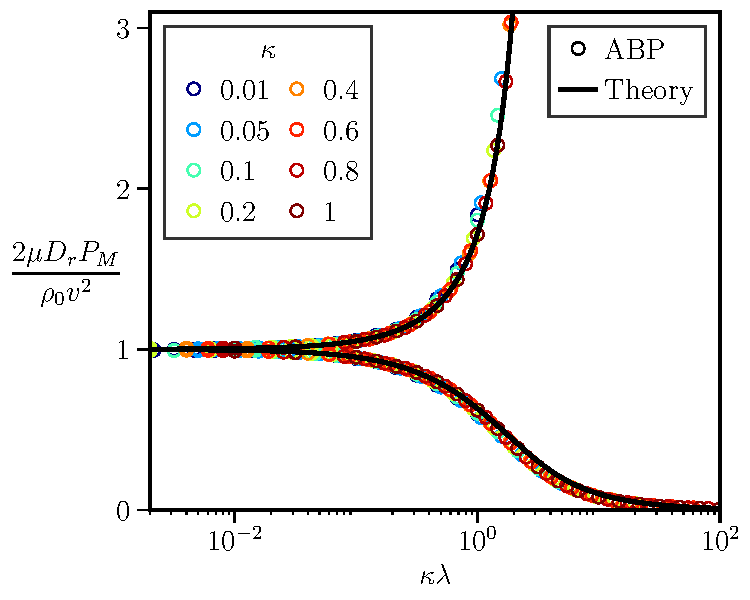
\includegraphics[width=0.4\linewidth]{fig1_2a_pour_yariv}
%	\caption{Test figure.}
%\end{figure}
%

%It all becomes clear if you read \cite{Fily2017}.


%==========================================================================
%==========================================================================
% Appendices

%\appendix

\printindex

%\section{An appendix}

%==========================================================================

%\section{An other appendix}

%==========================================================================
%==========================================================================
% Bibliography.

% Some other possible styles: abbrv, acm, alpha, apalike, ieeetr, plain, siam, unsrt
\bibliographystyle{plain}
\bibliography{honors_thesis_bibliography} % Use the name of you bibliography file. Omit the ".bib" extension.

\end{document}

